% Foliensatz: "AFu-Kurs nach DJ4UF" von DK0TU, Amateurfunkgruppe der TU Berlin
% Lizenz: CC BY-NC-SA 3.0 de (http://creativecommons.org/licenses/by-nc-sa/3.0/de/)
% Autoren: Sebastian Lange <dl7bst@dk0tu.de>
% Korrekturen: Lars Weiler <dc4lw@darc.de>

\documentclass[aspectratio=169]{beamer}

\usepackage[ngerman]{babel} % deutsche Worttrennung etc.
\usepackage[utf8]{inputenc} % UTF8 Text

\usepackage[super, comma, numbers, square, sort]{natbib}

\usepackage{hyperref}       % Hyperref Package für bessere Referenzen (todo)
\hypersetup{
	colorlinks=false,       %   false: boxed links; true: colored links
    %linkcolor=white,       %   color of internal links (change box color with linkbordercolor)
    citecolor=red,          %   color of links to bibliography
    filecolor=white,        %   color of file links
    urlcolor=blue           %   color of external links
}

\usepackage{multirow}
\usepackage{wasysym}  % Math Symbols like \permil
%\usepackage{colortbl}
%\usepackage{subscript}
%\usepackage{caption}
%\usepackage{setspace}
%\usepackage{xcolor}        % benutze CodeListe

% Footnote
%\usepackage{hanging}
%
%\setbeamertemplate{footnote}{%
%  \hangpara{2em}{1}%
%  \makebox[2em][l]{\insertfootnotemark}\footnotesize\insertfootnotetext\par%
%}


%\usepackage{pgf}
%\usepackage{tikz}
%\usetikzlibrary{arrows,automata}
%\usetikzlibrary{positioning}
%
%\tikzset{
%    state/.style={
%           rectangle,
%           rounded corners,
%           draw=black, very thick,
%           minimum height=2em,
%           minimum width=2pt,
%           inner sep=2pt,
%           text centered,
%           },
%}

%\usepackage{listings}
%\lstset{basicstyle=\small, numberstyle=\tiny, extendedchars=true, numbers=left, numbersep=5pt}
%\lstset{showtabs=false, showspaces=false, showstringspaces=false}
%%\lstset{backgroundcolor=\color{white!75!lightgray}, , frame=single}
%%\lstset{backgroundcolor=\color{white}}
%%\lstset{backgroundcolor=none}
%\lstset{keywordstyle=\color{blue!50!gray},  identifierstyle=\color{black}}
%\lstset{commentstyle=\color{green!50!gray}, stringstyle=\color{red!50!gray}}
%\lstset{language=C, fontadjust=true, tabsize=2, breaklines=true}
%\lstset{backgroundcolor=\color{white!75!lightgray}, caption=\lstname, frame=single}
%\lstset{emphstyle=\color{black}\fbox}
%
%% Keine "Listing:"-Caption
%\captionsetup{labelformat=empty,labelsep=none}
%
%% für mathematische Umgebungen
%\usepackage{amsmath,amsfonts,amssymb}
%
%\lstdefinestyle{Bash}{
%language=Bash,
%frame=single,
%rulecolor=\color{black},
%backgroundcolor=\color{gray!50},
%keywordstyle=\color{black},
%identifierstyle=,
%commentstyle=\color{black},
%stringstyle=\color{magenta!65!white},
%showstringspaces=false,
%basicstyle=\footnotesize\ttfamily\color{black},
%numbers=none,
%breaklines=true,
%captionpos=b
%}

%\usepackage{listings}
%
%\lstdefinestyle{basic}{
%    captionpos=t,%
%    basicstyle=\footnotesize\ttfamily,%
%    numberstyle=\tiny,%
%    numbers=left,%
%    stepnumber=1,%
%    frame=single,%
%    showspaces=false,%
%    showstringspaces=false,%
%    showtabs=false,%
%    %
%    keywordstyle=\color{blue},%
%    identifierstyle=,%
%    commentstyle=\color{gray},%
%    stringstyle=\color{magenta}%
%}



% fließende Boxen haben keinen Abstand
%\fboxsep0mm

% inkludiere Creative Commons Helper
%%%%%%%%%%%%%%%%%%%%%%%%%%%%%%%%%%%%%%%%%%%%%%%%%%%%%%%%%%%%%%%%
%% ccBeamer 0.1, 2007-07-02                                   %%
%% Written by Sebastian Pipping <webmaster@hartwork.org>      %%
%% ---------------------------------------------------------- %%
%% Licensed under Creative Commons Attribution-ShareAlike 3.0 %%
%% http://creativecommons.org/licenses/by-sa/3.0/             %%
%%%%%%%%%%%%%%%%%%%%%%%%%%%%%%%%%%%%%%%%%%%%%%%%%%%%%%%%%%%%%%%%


%% Images
\newcommand{\CcImageBy}[1]{%
	
\includegraphics[scale=#1]{texdata/creative_commons/cc_by_30.pdf}%
}
\newcommand{\CcImageCc}[1]{%
	
\includegraphics[scale=#1]{texdata/creative_commons/cc_cc_30.pdf}%
}
\newcommand{\CcImageDevNations}[1]{%
	
\includegraphics[scale=#1]{texdata/creative_commons/cc_dev_nations_30.pdf}%
}
\newcommand{\CcImageNc}[1]{%
	
\includegraphics[scale=#1]{texdata/creative_commons/cc_nc_30.pdf}%
}
\newcommand{\CcImageNd}[1]{%
	
\includegraphics[scale=#1]{texdata/creative_commons/cc_nd_30.pdf}%
}
\newcommand{\CcImagePd}[1]{%
	
\includegraphics[scale=#1]{texdata/creative_commons/cc_pd_30.pdf}%
}
\newcommand{\CcImageSa}[1]{%
	
\includegraphics[scale=#1]{texdata/creative_commons/cc_sa_30.pdf}%
}
\newcommand{\CcImageSampling}[1]{%
	
\includegraphics[scale=#1]{texdata/creative_commons/cc_sampling_30.pdf}%
}
\newcommand{\CcImageSamplingPlus}[1]{%
	
\includegraphics[scale=#1]{texdata/creative_commons/cc_sampling_plus_30.pdf}%
}


%% Groups
\newcommand{\CcGroupBy}[2]{% zoom, gap
	\CcImageCc{#1}\hspace*{#2}\CcImageBy{#1}%
}
\newcommand{\CcGroupByNc}[2]{% zoom, gap
	\CcImageCc{#1}\hspace*{#2}\CcImageBy{#1}\hspace*{#2}\CcImageNc{#1}%
}
\newcommand{\CcGroupByNcNd}[2]{% zoom, gap
	\CcImageCc{#1}\hspace*{#2}\CcImageBy{#1}\hspace*{#2}\CcImageNc{#1}\hspace*{#2}\CcImageNd{#1}%
}
\newcommand{\CcGroupByNcSa}[2]{% zoom, gap
	\CcImageCc{#1}\hspace*{#2}\CcImageBy{#1}\hspace*{#2}\CcImageNc{#1}\hspace*{#2}\CcImageSa{#1}%
}
\newcommand{\CcGroupByNd}[2]{% zoom, gap
	\CcImageCc{#1}\hspace*{#2}\CcImageBy{#1}\hspace*{#2}\CcImageNd{#1}%
}
\newcommand{\CcGroupBySa}[2]{% zoom, gap
	\CcImageCc{#1}\hspace*{#2}\CcImageBy{#1}\hspace*{#2}\CcImageSa{#1}%
}
\newcommand{\CcGroupDevNations}[2]{% zoom, gap
	\CcImageCc{#1}\hspace*{#2}\CcImageDevNations{#1}%
}
\newcommand{\CcGroupNcSampling}[2]{% zoom, gap
	\CcImageCc{#1}\hspace*{#2}\CcImageNc{#1}\hspace*{#2}\CcImageSampling{#1}%
}
\newcommand{\CcGroupPd}[1]{% zoom
	\CcImagePd{#1}%
}
\newcommand{\CcGroupSampling}[1]{% zoom
	\CcImageSampling{#1}%
}
\newcommand{\CcGroupSamplingPlus}[1]{% zoom
	\CcImageSamplingPlus{#1}%
}


%% Text
\newcommand{\CcLongnameBy}{Attribution}
\newcommand{\CcLongnameByNc}{Attribution-NonCommercial}
\newcommand{\CcLongnameByNcNd}{Attribution-NoDerivs}
\newcommand{\CcLongnameByNcSa}{Attribution-NonCommercial-ShareAlike}
\newcommand{\CcLongnameByNd}{Attribution-NoDerivs}
\newcommand{\CcLongnameBySa}{Attribution-ShareAlike}

\newcommand{\CcNote}[1]{% longname
	This work is licensed under the \textit{Creative Commons #1 3.0 License}.%
}


% generelles Thema auswählen
\usetheme{Goettingen} %Berlin spart ohne Sidebar allerdings angenehm Platz
% AnnArbor | Antibes | Bergen | Berkeley | Berlin | Boadilla | boxes | CambridgeUS | Copenhagen | Darmstadt | default | Dresden | Frankfurt | Goettingen | Hannover | Ilmenau | JuanLesPins | Luebeck | Madrid | Malmoe | Marburg | Montpellier | PaloAlto | Pittsburgh | Rochester | Singapore | Szeged | Warsaw

% Farben wählen
\usecolortheme{beetle}
% beaver | beetle | crane | default | dolphin | dove | fly | lily | orchid | rose | seagull | seahorse | sidebartab | structure | whale | wolverine

% Setze alle Farben auf Grau und Weiß
%\definecolor{craneorange}{RGB}{64,64,64}
%\definecolor{craneblue}{RGB}{255,255,255}

% Schriftart wählen
\usefonttheme{default}
% default | professionalfonts | serif | structurebold | structureitalicserif | structuresmallcapsserif

% Innere Themen(Kopf-, Fuß-, Sidebar usw)
%\useinnertheme{default}
\useinnertheme{circles}
% default | inmargin | rectangles | rounded | circles

% Äußere Themen (Anordnung der inneren, grenzen der Folien etc.)
\useoutertheme{infolines}
% default | infolines | miniframes | shadow | sidebar | smoothbars | smoothtree | split | tree

% Deaktiviere Navigations-Symbole ({} -> leer)
\setbeamertemplate{navigation symbols}{}
%\setbeamertemplate{navigation symbols}{\large \ifnum \insertframenumber <10 0\fi\insertframenumber/\inserttotalframenumber\vspace*{0.2ex}}

% Zeige ein Hintergrundbild
\setbeamertemplate{background canvas}{
        \hspace*{-2.0cm}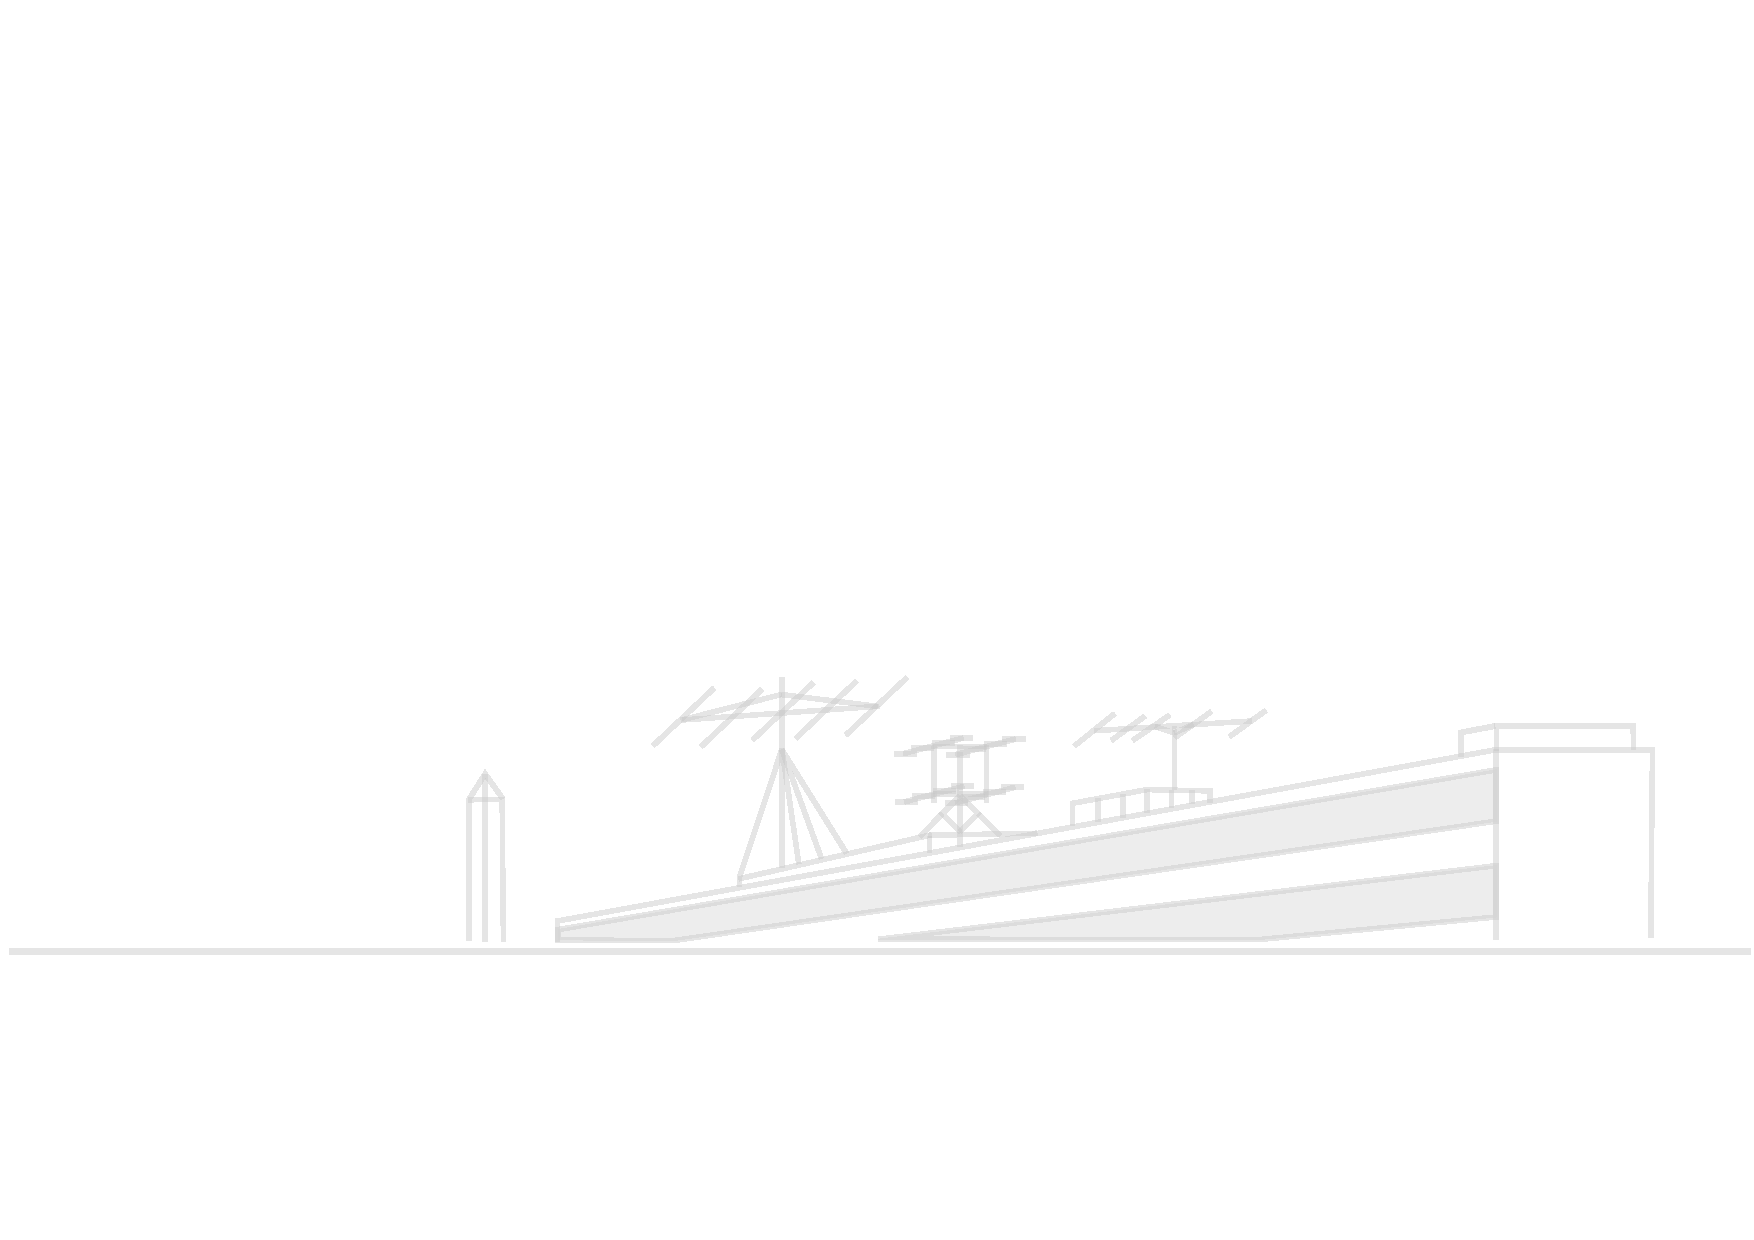
\includegraphics[width=17.8cm]{texdata/dk0tu_rooftop_background.pdf}
}

% Foliennummer einfügen
\setbeamertemplate{footline}[frame number]
%\setbeamertemplate{footline}{}

% Ändere das Zeichen vor jedem item
%\setbeamertemplate{itemize item}{\color{craneorange}$\blacktriangleright$}
%\setbeamertemplate{itemize subitem}{\color{craneorange}$\triangleright$}
%\setbeamertemplate{itemize subsubitem}{\color{craneorange}$\blacktriangleright$}

% Ändert die Blöcke 
\setbeamertemplate{blocks}[rounded][shadow=true]
% default | rounded [shadow=true|false]

%
% Eigene Kommandos
%

% Hack to get natbib and beamer working together. "The beamer user guide suggests
% that only the manual bibliography entry approach is supported"
% on some system it works out of the box, sometimes you need the hack :-(
% so check it --dl7bst
\ifdefined\newblock
    \relax
\else
    \newcommand{\newblock}{}
\fi

% \includedia command to generate png out of a dia file
% NEEDS installed dia and pdflatex option --shell-escape
\newcommand{\includedia}[1]{
    \immediate\write18{/usr/bin/dia #1.dia -e #1_diatmp.png -t png}
}

% RICHIG GROSSER FONT!
\newfont{\bigfont}{cmr10 at 144pt}
\newfont{\smallfont}{cmr10 at 8pt}

% Römische Ziffern
\makeatletter
\newcommand{\rmnum}[1]{\romannumeral #1}
\newcommand{\Rmnum}[1]{\expandafter\@slowromancap\romannumeral #1@}
\makeatother

% Schwarze Überschrift
%\setbeamercolor{frametitle}{fg=black}
%\setbeamercolor{title}{fg=black}

% Item- und Box-Farben
\definecolor{deepBlue}{HTML}{000066}
\setbeamercolor{itemize item}{fg=deepBlue}
\setbeamercolor{itemize subitem}{fg=deepBlue}
\setbeamercolor{description item}{fg=deepBlue}
\setbeamercolor{block title}{fg=deepBlue!100, bg=blue!15}
\setbeamercolor{block body}{fg=black, bg=blue!5}
\setbeamercolor{block title alerted}{fg=deepBlue, bg=red!75}
\setbeamercolor{block body alerted}{fg=black, bg=red!15}
\setbeamercolor*{block title example}{fg=blue!50, bg=blue!10}
\setbeamercolor*{block body example}{fg= blue, bg=blue!5}

%\setbeamercolor{section in head/foot}{parent=palette primary}
%\setbeamercolor{subsection in head/foot}{parent=palette secondary}
%\setbeamercolor{sidebar}{fg=darkblue,bg=yellow!90!orange}
%\setbeamercolor{title in sidebar}{fg=darkblue}
%\setbeamercolor{author in sidebar}{fg=darkblue}
%\setbeamercolor{section in sidebar}{fg=darkblue!10!black}
%\setbeamercolor{subsection in sidebar}{fg=darkblue!50!black}

% Titlepage Infos
\title{AFu-Kurs nach DJ4UF}
\author[DKØTU]{DKØTU\\ \footnotesize{Amateurfunkgruppe der TU Berlin}}
\institute[DKØTU]{\url{http://www.dk0tu.de} }

% PDF-Eigenschaften
\subject{DK0TU-Amateurfunkkurs nach DJ4UF}
\keywords{Amateurfunk Kurs HAM Radio Course CC-BY-NC-SA OpenSource TU Berlin DK0TU}

\subtitle{Betriebstechnik/Vorschriften 09: \\
  Betriebsarten, Sendearten, Frequenzen \\[2em]}
\date{Stand 18.09.2017}
 \begin{document}

\begin{frame}
    \titlepage
    \vfill
    \begin{center}
        \ccbyncsaeu\\
        {\tiny This work is licensed under the \em{Creative Commons Attribution-NonCommercial-ShareAlike 3.0 License}.}\\[0.5ex]
         \tiny Amateurfunkgruppe der Technische Universität Berlin (AfuTUB), DKØTU
         %\includegraphics[scale=0.5]{img/DK0TU_Logo.pdf}
    \end{center}
\end{frame}


%todo Struktur nach Moltrecht, aber sehr komisch
%     Besser Top-Down: ITU ... AFuV ... HAM Conventions

\section{Einleitung}

\begin{frame}
  \frametitle{Einleitung: International}

  Internationaler Frequenzbereichszuweisungsplan:
  \emph{ITU\footnote{International Telecommunication Union.
  Gesetzesgrundlagen siehe Lektion \texttt{BV06}: ITU, CEPT, AFuV, \ldots} Frequency
  Allocation Table}

  \begin{itemize}
    \item enthält die Frequenzbereichszuweisungen aller Funkdienste in
      verschiedenen Funkregionen der Erde\footnote{Regionen siehe Lektion \texttt{BV06}}
  \end{itemize}

\end{frame}

\begin{frame}
  \frametitle{Einleitung: National}

  National geltendes Recht (in DL \texttt{AFuV}):

  \begin{itemize}
    \item Anlage 1 der \texttt{AFuV} regelt Nutzungsbedingungen und Frequenzbereiche
    \item welche Bereiche von wem wie genutzt? \\
      Frequenzen, Bandbreiten, Leistung, \ldots
    \item folglich: Nicht alle Bereiche der RR (VO Funk) dürfen automatisch
      verwendet werden
    \item Bandgrenzen HF bis 13cm muss man lernen\footnote{bei vielen
      Prüfungsfragen hilft einfache Faustformel $MHz = \frac{300}{Meter}$}
  \end{itemize}

\end{frame}

\begin{frame}
  \frametitle{Bänder}
  Bandgrenzen für die Prüfung relevant

  \begin{center}
    {\footnotesize
    \begin{tabular}{r|r|r|l}\hline
      \textbf{Meter} & \textbf{min. QRG} & \textbf{max. QRG} & \textbf{Klasse} \\\hline\hline
      160m &   1810 kHz &   2000 kHz & A + E \\
      80m  &   3500 kHz &   3800 kHz & A + E \\
      40m  &   7000 kHz &   7200 kHz & A \\
      30m  &  10100 kHz &  10150 kHz & A \\
      20m  &  14000 kHz &  14350 kHz & A \\
      17m  &  18068 kHz &  18168 kHz & A \\
      15m  &  21000 kHz &  21450 kHz & A + E \\
      12m  &  24890 kHz &  24990 kHz & A \\
      10m  &  28000 kHz &  29700 kHz & A + E \\
      6m   &  50,08 MHz &     51 MHz & A \\
      2m   &    144 MHz &    146 MHz & A + E \\
      70cm &    430 MHz &    440 MHz & A + E \\
      23cm &   1240 MHz &   1300 MHz & A \\
      13cm &   2320 MHz &   2450 MHz & A \\\hline
    \end{tabular}
    }
  \end{center}

  Weitere Bänder möglich, z.B. 60m bei WRC-15 für Amateurfunk freigegeben.
\end{frame}


\begin{frame}
  \frametitle{Einleitung: Vereinbarungen der HAMs}

  International:

  \begin{itemize}
    \item IARU\footnote{International Amateur Radio Union} legt
      Nutzungs\emph{empfehlungen} der Funkamateure untereinander fest
  \end{itemize}

  Lokale Absprachen, z.\,B.

  \begin{itemize}
    \item Club QRGs
    \item Lokalrunden
    \item Rundsprüche
    \item \ldots
  \end{itemize}

\end{frame}

\section[Übertra\-gungs\-technik]{Übertragungstechnik}

\begin{frame}
  \frametitle{Übertragungstechnik}

  \begin{center}
    Modulationsarten, Betriebsarten $\Rightarrow$ Sendearten\footnote{später
    in \texttt{E14}, \texttt{E16} und \texttt{BV12}}
  \end{center}

\end{frame}

\begin{frame}
  \frametitle{Modulationsarten}

  Radio Regulations verwendet offizielle Codierung von Aussendungen als
  neunstelligen Code \texttt{BBBB\,MSI\,DX}: \\[2em]

  \begin{description}
    \item[BBBB] vier Stellen Bandbreite
    \item[MSI] drei Stellen Sendeart (Modulationsart, Signalart,
      Informationsgehalt)
    \item[DX] ggf. zwei weitere Stellen für Signaleinzelheiten
      (Detaillierung, Multiplexverfahren)
  \end{description}

\end{frame}

\begin{frame}
  \frametitle{Sendearten: Amateurfunk}

  Amateurfunk: drei Kennzeichen für die Modulationsart ausreichend (\texttt{MSI})

  %todo enumerate color broken
  \begin{enumerate}
    \item Modulationsart
    \item Signalart, die den Hauptträger moduliert
    \item Art der Informationen
  \end{enumerate}

  %todo Tabellen http://de.wikipedia.org/wiki/Modulationsart

\end{frame}

\begin{frame}[allowframebreaks]
  \frametitle{Sendearten: Schlüsselzeichen}

  \begin{block}{Modulationsart des Hauptträgers}
    \begin{description}
      \item[A] Amplitudenmodulation
      \item[J] SSB (AM, Seitenband mit unterdrücktem Träger)
      \item[F] Winkelmodulation, Frequenzmodulation
    \end{description}
  \end{block}

  \begin{block}{Signalart}
    \begin{description}
      \item[1] Einkanaliges quantisiertes Signal ohne Hilfsträger
      \item[2] Einkanaliges quantisiertes Signal mit einem Hilfsträger
      \item[3] Einkanaliges Analogsignal
    \end{description}
  \end{block}

  \begin{block}{Informationsart}
    \begin{description}
      \item[A] Morsetelegrafie
      \item[B] Telegrafie für maschinellen Empfang (Teletype)
      \item[C] Fax
      \item[D] Daten, Telemetrie, Fernsteuerung
      \item[E] Telefonie, Rundfunk
      \item[F] Fernsehsignal
    \end{description}
  \end{block}

\end{frame}

\begin{frame}
  \frametitle{Sendearten: Beispiele}

  \begin{exampleblock}{Beispiele für Sendearten}
    \begin{description}
      \item[A1A] CW
      \item[F2A] CW via FM-Hilfsträger
      \item[F3E] FM
      \item[J3E] SSB
      \item[J2B] RTTY
      \item[J2B] Pactor
    \end{description}
  \end{exampleblock}

  Übersichtliche Liste: \ExternalLink\url{https://de.wikipedia.org/wiki/Modulationsart}

\end{frame}

\begin{frame}
  \begin{figure}
    \begin{center}
      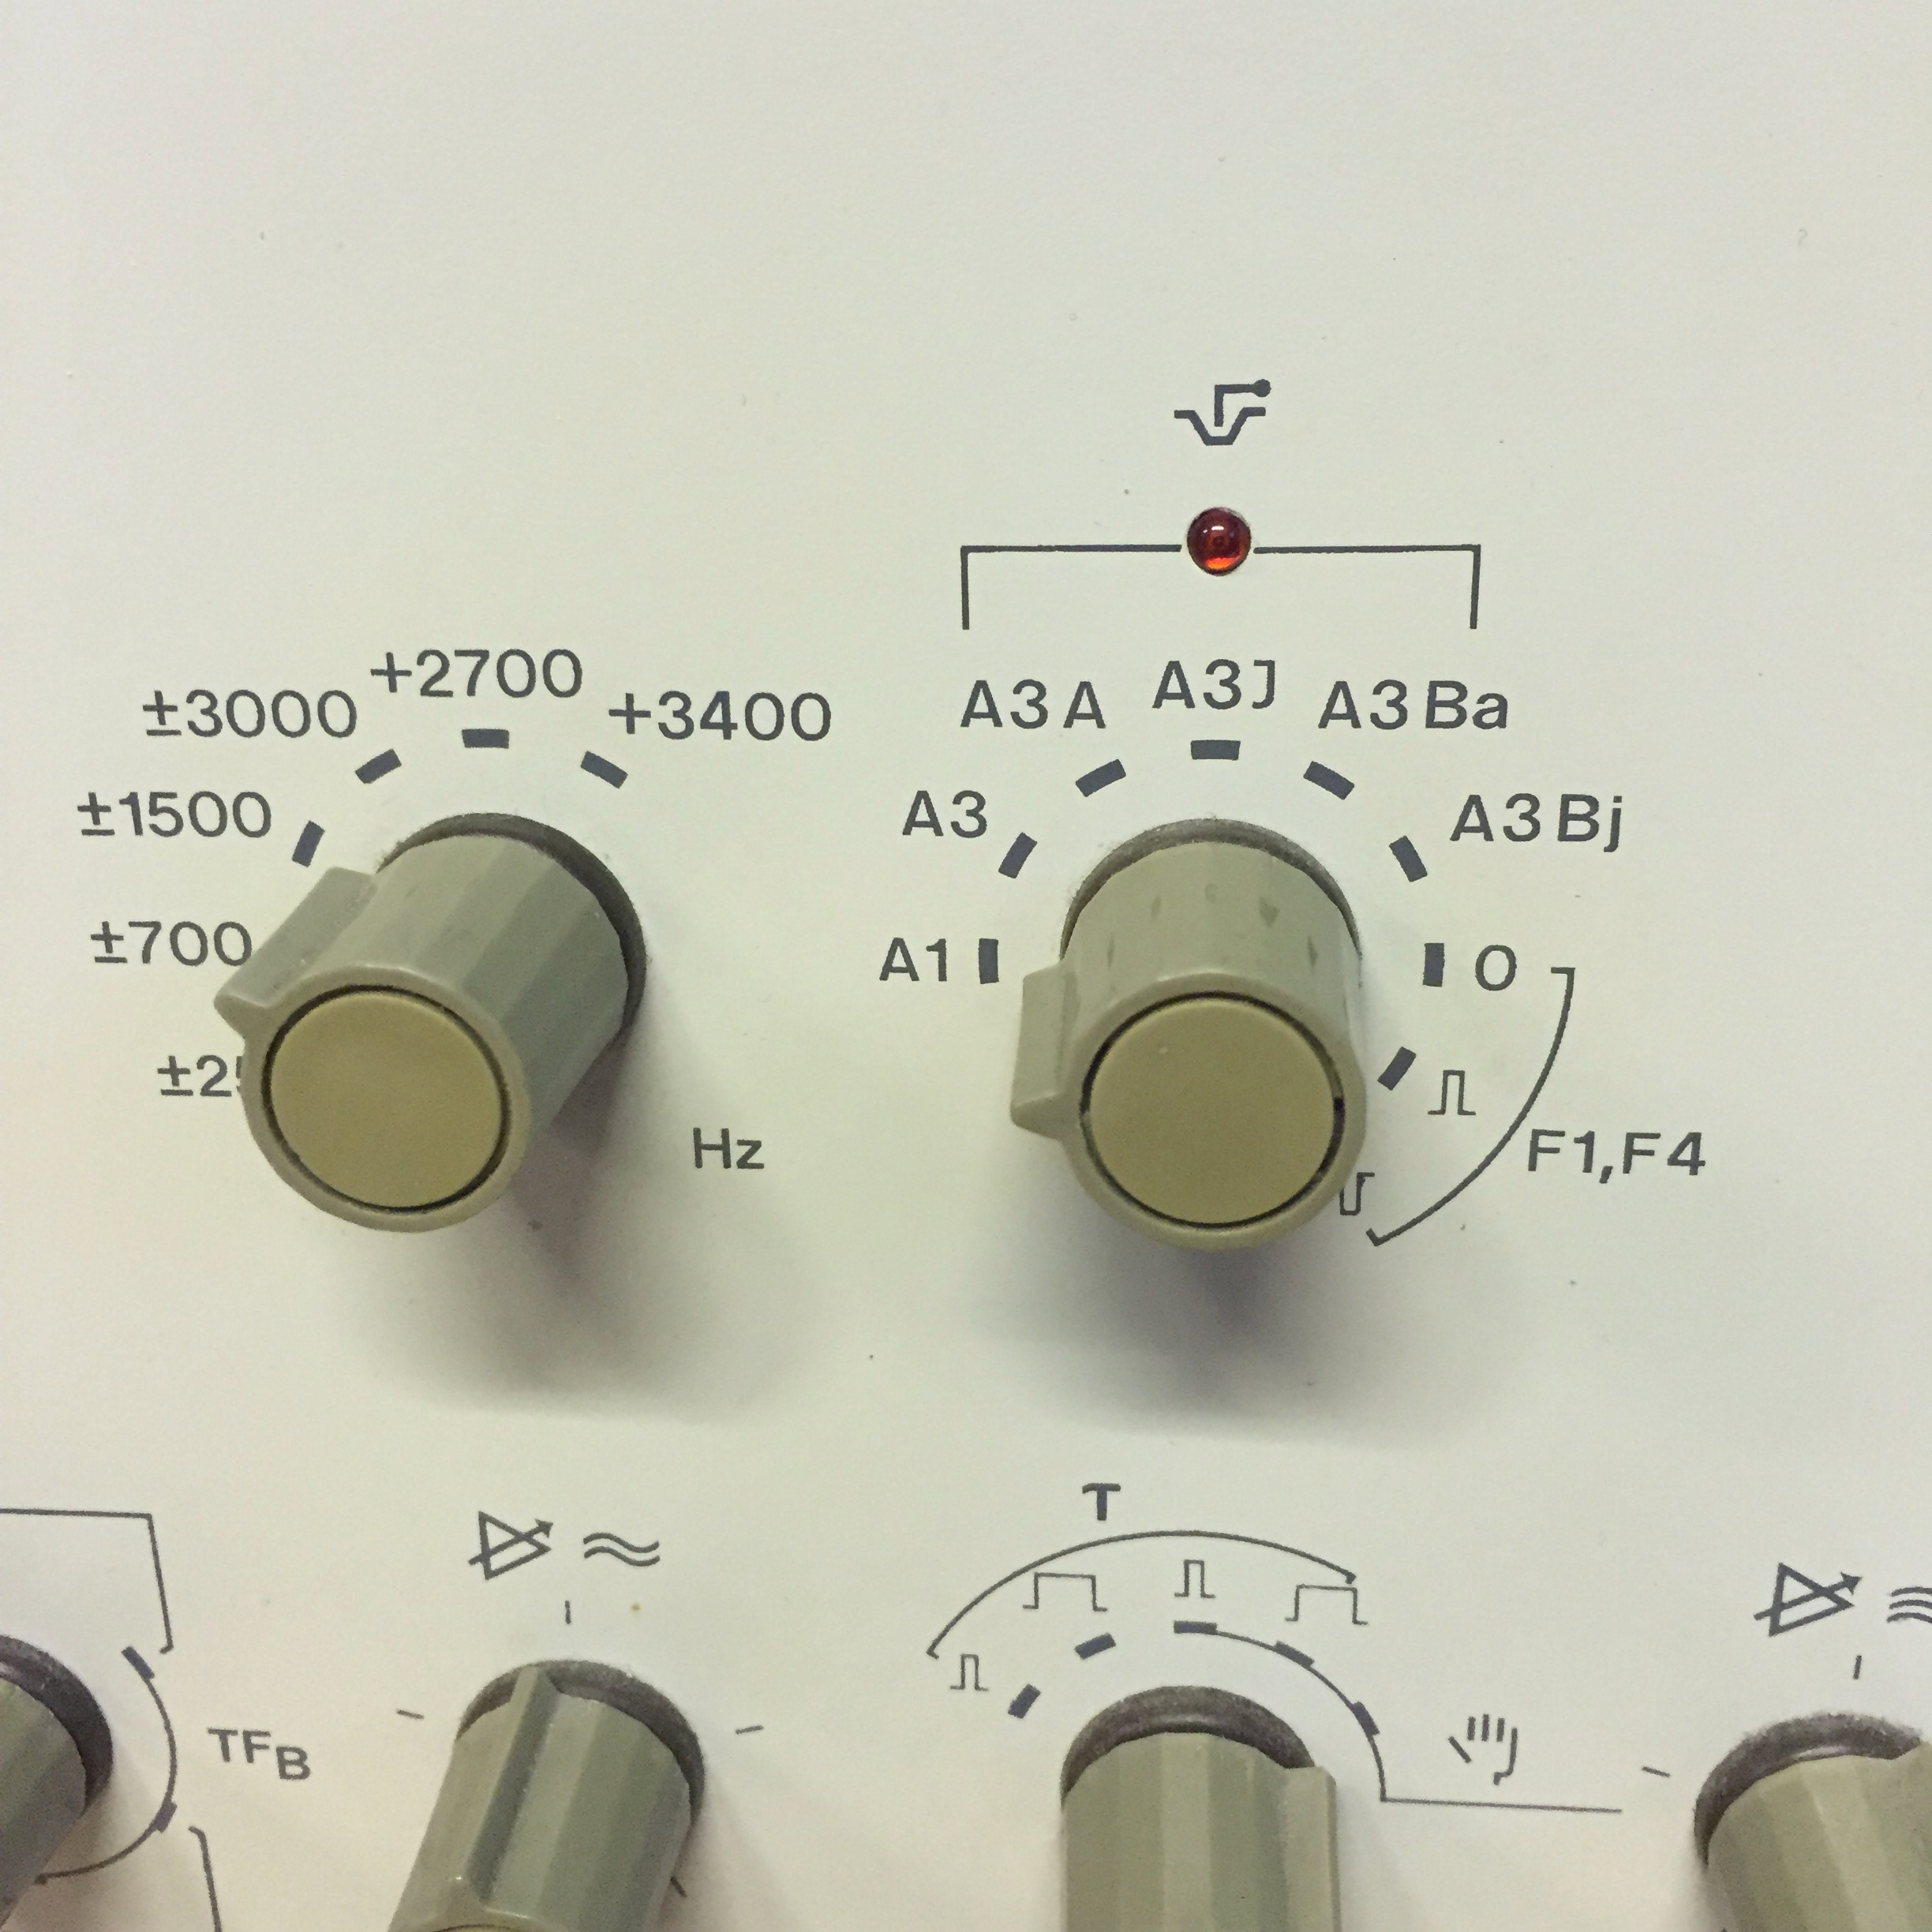
\includegraphics[width=\textwidth,height=.75\textheight,keepaspectratio]{bv09/RFT_EKD300.jpg}
    \end{center}
    \caption{Einstellung der Sendeart am RFT EKD300 Kurzwellenempfänger}
  \end{figure}
\end{frame}

\begin{frame}
  \frametitle{Bandbreiten}

  \begin{block}{Bandbreiten}
    \begin{description}
      \item[A1A] 0,1\ldots0,5 kHz
      \item[F1B] 0,5 kHz
      \item[A3E] 5 kHz
      \item[F3E] 12 kHz
      \item[J3E] 2,4 kHz (2,7 kHz)
    \end{description}
  \end{block}

  Weitere Einschränkungen, z.B. 160m-Band kein FM.

\end{frame}


\section{IARU-Bandplan (Kurzwelle)}

\begin{frame}
  \frametitle{IARU-Bandplan (Kurzwelle)}

  % todo Bandplan vorher drucken

  \begin{itemize}
    \item Bei uns Region 1 -- remember?
    \item Aufteilung: Vereinbarung der HAMs untereinander mit ``Charakter
      einer Empfehlung''
    \item CW überall erlaubt, aber am Bandanfang exklusiv
    \item auch hier: Frequenzen kann man sich etwas herleiten, aber im
      Prinzip muss man Lernen, sorry
    \item Ansonsten: Lösung ist immer ``Ich schaue im aktuellen HF-Bandplan
      der IARU nach \ldots'' ;-)
  \end{itemize}

\end{frame}

%\begin{frame}
%  \begin{center}
%    \begin{tabular}{l||p{.8\textwidth}}\hline
%      \textbf{BC214} & \textbf{Aus welchem Grund sollten Sie in der Dunkelheit und im Winter auch tagsüber im Bereich von 3500-3510 kHz keine innerdeutschen oder innereuropäischen Telegrafie-QSOs durchführen?} \\ \hline\hline
%      A \only<2>\checkmark & Im IARU-Region-1-Kurzwellenbandplan ist dieser Bereich als ``CW DX'' ausgewiesen und sollte für interkontinentale Verbindungen freigehalten werden. \\\hline
%      B & Gemäß Frequenzbereichszuweisungsplan ist dieser Bereich auch kommerziellen Stationen zugewiesen und muss nachts und im Winter freigehalten werden. \\\hline
%      C & Im IARU-Region-1-Kurzwellenbandplan ist dieser Bereich für Digimode-Betriebsarten ausgewiesen und sollte von CW-Stationen nicht benutzt werden. \\\hline
%      D & Weil dieser Bereich im Ausland auch für Rundfunkstationen ausgewiesen ist und daher nachts und im Winter durch den Amateurfunkdienst nicht genutzt werden darf. \\\hline
%    \end{tabular}
%  \end{center}
%\end{frame}

\subsection{Aktivitätszentren}

\begin{frame}
  \frametitle{Aktivitätszentren}

  \begin{itemize}[<+->]
    \item QRP -- wozu?
    \item anbei: Verwendung von \texttt{/qrp} nicht offiziell, aber geduldet
    \item Bildübertragung
    \item Notfunk
    \item Frequenzbereiche bevorzugt Funkverkehr in digitalen Betriebsarten
  \end{itemize}

\end{frame}

\subsection{Seitenbänder}

\begin{frame}
  \frametitle{Seitenbänder}

  Konvention: \bigskip

  \begin{itemize}
    \item [$<$] $10 MHz$ LSB\footnote{Lower Side Band $\rightarrow$ \texttt{E14}} \\[1em]
    \item [$>$] $10 MHz$ USB\footnote{Upper Side Band $\rightarrow$ \texttt{E14}} \\[3em]
  \end{itemize}

  Nicht mit deutschen Abkürzungen (USB, OSB) verwechseln!

\end{frame}

\subsection{Betriebstechniken}

\begin{frame}
  \frametitle{Betriebstechniken}

  \begin{itemize}
    \item QRGs werden ``occupied'' -- man fragt vorher, ob sie frei sind
    \item für höhere Bänder gibt es Anruf\/frequenzen, weil diese groß sind und oft mit
      Richtantennen gearbeitet wird
      \begin{itemize}
        \item nach Kontaktaufnahme sofort QSY
      \end{itemize}
    \item Satellitenfunkbetrieb
      \begin{itemize}
        \item Uplink-/Downlink-Bereiche
        \item manchmal FM, manchmal SSB mit LSB im Uplink und USB im Downlink
        \item auch mit Handfunkgeräten (HFG) frei halten\footnote{freie
          Sicht direkt zum Satelliten; selbst Signale mit wenigen $mW$
          können die $400km$ vom/zum Satelliten gehört werden}!
        \item auch hier: Bereiche leider Lernstoff
      \end{itemize}
  \end{itemize}

\end{frame}

\section[Frequenz\-nutzungs\-plan]{Frequenznutzungsplan}

\begin{frame}
  \frametitle{Frequenznutzungsplan}

  in Anlage 1 der \texttt{AFuV}\cite{afuv}: \\[1em]

  %todo Frequenznutzungsplan ggf. in die Folien mit einbinden

  Ausführlichen Nutzungsbedingungen und die ausgewiesenen Frequenzbereiche für
  den Amateurfunkdienst.

  \begin{itemize}
    \item maximal zulässigen Sender- bzw. Strahlungsleistungen
    \item erlaubte Frequenzbereiche
    \item aufgegliedert nach Zeugnisklassen
    \item Einzelheiten über Aufteilung und Nutzung im
      Frequenznutzungsplan und im Frequenzbereichszuweisungsplan
  \end{itemize}

\end{frame}

\begin{frame}
  \frametitle{Frequenznutzungsplan: Lesehilfen}

  \begin{itemize}[<+->]
    \item Status: Der (S)ekundärfunkdienst hat im Störungsfall gegenüber einem
      (P)rimärfunkdienst eingeschränkte Nutzungsrechte.
    \item ISM\footnote{Industrial, Scientific and Medical Band}: Dieser
      Frequenzbereich wird für industrielle, wissenschaftliche,
      medizinische, häusliche oder ähnliche Anwendungen mitbenutzt.
      \begin{itemize}
        \item Welche ISM-Dienste kennt ihr?
      \end{itemize}
    \item richtige Anfangs- und Endfrequenzen und Bandbreiten muss man
      leider teilweise lernen, aber helfen später im Betrieb gut weiter
  \end{itemize}

\end{frame}

\begin{frame}
  \frametitle{Frequenznutzungsplan: Fragen}

  ``Funfacts'':

  \begin{itemize}
    %\item Bei 135,7-137,8 kHz und 1810-1850 kHz beträgt die zulässige maximale
    %      Bandbreite nur 800 Hz
    \item CB-Funkverkehr darf nur mit speziell für diesen Frequenzbereich
      hergestellten Geräten durchgeführt werden, für die eine
      Konformitätsbewertung oder Zulassung vorliegt.
    \item Betriebsfunk: Nein. Außerhalb des Amateurfunks dürfen nur zugelassene Geräte oder
      konformitätsbewertete Geräte benutzt werden.
  \end{itemize}

\end{frame}

\section{Lernhinweise}

\begin{frame}
  \frametitle{Lernhinweise}

  Die Frequenzbereiche gehören leider mit zu dem stupidesten Lernstoff für die
  Prüfung. Tipps:

  \begin{itemize}
    \item Don't Panic! ;-)
    \item bei der Prüfungssimulation am Anfang die Frequenzfragen mit Hilfe
      der Bandpläne beantworten und sacken lassen
    \item viele Fragen sind auch über die ``Faustformel'' zu lösen
    \item Antworten mit ``ich schau in Regelwerken nach'' sind immer gut
  \end{itemize}

\end{frame}

\begin{frame}
  \frametitle{Hausaufgaben}

  \begin{alertblock}{Fakultative Hausaufgaben}
    \begin{itemize}
      \item Fragenkatalog Betrieb und Vorschriften, Kapitel 2.3 ``Frequenzbereiche und IARU-Bandpläne'', bestehend aus 2.3.1 ``Frequenzbereiche des Amateurfunkdienstes'', 2.3.2 ``IARU-Bandpläne''.
      \item Fragenkatalog Betrieb und Vorschriften, Kapitel 2.2.4 ``Bezeichnungen der Aussendungen (Sendearten)''
    \end{itemize}
  \end{alertblock}
\end{frame}

\renewcommand{\refname}{Referenzen}

\begin{frame}
  \frametitle{Referenzen/Links}
  \hypertarget{refs}{}
  \footnotesize

  \begin{thebibliography}{}
    \bibitem{dj4uf} Moltrecht B/V 09: \\
      \url{https://www.darc.de/der-club/referate/ajw/lehrgang-bv/bv09/}
    \bibitem{wp}    Wikipedia DE: \\
      \url{http://de.wikipedia.org/wiki/Frequenzzuteilung} \\
      \url{http://de.wikipedia.org/wiki/Amateurfunkband} \\
      \url{http://de.wikipedia.org/wiki/Betriebsart_\%28Amateurfunk\%29} \\
      \url{http://de.wikipedia.org/wiki/Modulationsart}
    \bibitem{frqs}  Frequenzplan der BRD von der BNetzA: \\
      \url{http://www.bundesnetzagentur.de/DE/Sachgebiete/Telekommunikation/Unternehmen_Institutionen/Frequenzen/Grundlagen/Frequenzplan/frequenzplan-node.html}
    \bibitem{darc}  Kurzwellenbandpläne der IARU Region 1: \\
      \url{http://www.darc.de/referate/hf/bandplaene/}
    \bibitem{afuv}  Verordnung zum Gesetz über den Amateurfunk: \\
      \url{http://www.gesetze-im-internet.de/afuv_2005/}
  \end{thebibliography}

\end{frame}

% Hier könnte noch eine Kontaktfolie stehen

\end{document}

